\documentclass{beamer}
\usepackage[utf8]{inputenc}
\usepackage[graphicx]

\author[Sowmya Vajjala]{Instructor: Sowmya Vajjala}


\title[LING 120]{LING 120: \\ Language and Computers}
\subtitle{Semester: FALL 2017}

\date{16 October 2017}

\institute{Iowa State University, USA}

%%%%%%%%%%%%%%%%%%%%%%%%%%%

\begin{document}

\begin{frame}\titlepage
\end{frame}

\begin{frame}
\frametitle{Outline}
\begin{enumerate}
\item Language and "secret writing" - an overview
\\ (based on the presentations by Jason Baldridge, Chris Brew and Marcus Dickinson)
\end{enumerate}
\end{frame}

\begin{frame}
\frametitle{Translation}
\begin{enumerate}
\item Is translation something that can be thought of as secret writing? How many of you think so? \pause
\item Does anyone of you have parents who spoke a language you did not know? \pause
\item Do you know about "Code Talkers"? \url{https://en.wikipedia.org/wiki/Code\_talker} \pause
\item Cryptography has in some ways helped us crack forgotten writing systems. 
\item communicate during war time.
\end{enumerate}
\end{frame}
%Exercise: texting, texting one,two,three in NACLO
%or: can translation be seen as a form of encryption? 

\begin{frame}
\frametitle{Branches of secret writing}
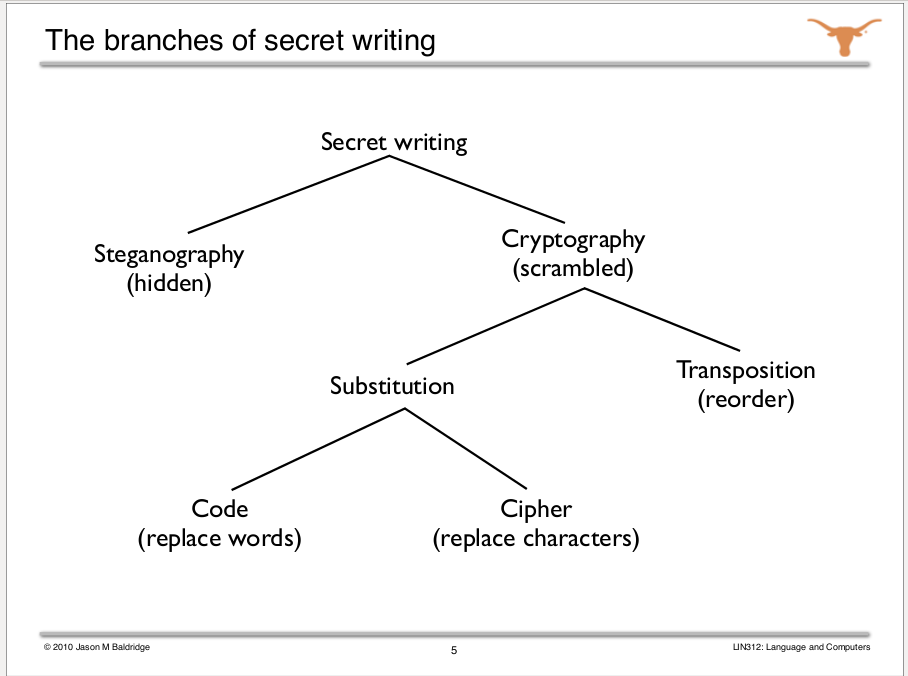
\includegraphics[width=0.9\textwidth]{crypto.png}
\end{frame}

\begin{frame}
\frametitle{Steganography}
\begin{itemize}
\item No encryption, just hiding the message in something (e.g., invisible ink)
\pause \item The story of Histiaeus:
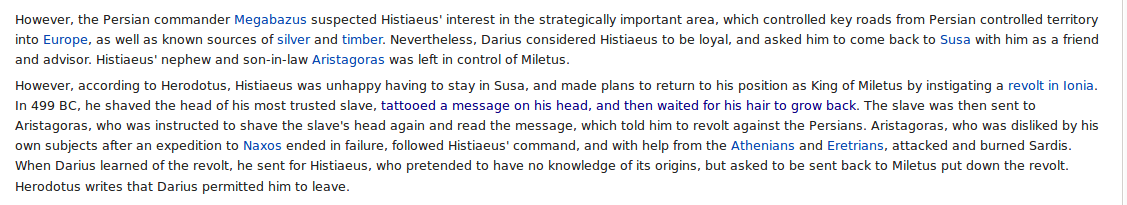
\includegraphics[width=0.9\textwidth]{histiaeus.png}
\item provides some security, but once detected, anyone can read. 
\end{itemize}
\end{frame}

\begin{frame}
\frametitle{Modern Steganography}
\begin{itemize}
\item Files (different forms of data) and Messages are hidden inside videos and pictures as well.
\\ 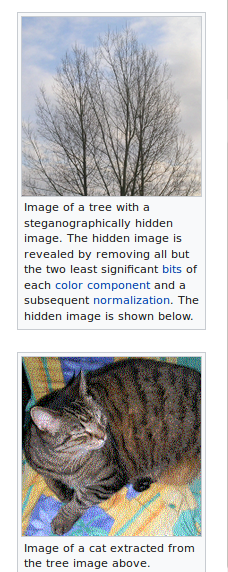
\includegraphics[width=0.2\textwidth]{steg.png}
\end{itemize}
\end{frame}

\begin{frame}
\frametitle{Cryptography}
\begin{itemize}
\item messages are not hidden - they can be seen by others, but they cannot make any sense out of it. 
\item messages are encrypted.
\item How?: simple encryptions are - interchanging letters, having a substitution map, or having a simple code (replace a with b, b with c, c with d and so on) \pause
\item What is cryptography? \pause - study of writing and breaking codes? 
\item what is the purpose? \pause - secure communication
\item where is it useful? \pause - paying with credit card online, transmitting our data across internet, passwords, military communication etc. (beyond language encryption)
\end{itemize}
\end{frame}

\begin{frame}
\frametitle{How does it work?}
\begin{itemize}
\item Encryption: some way to produce the cipher text
\item key: details of this encryption so that the receiver can decrypt
\item e.g., Caeser cipher: substitution cipher, where each letter in the original message is replaced with another letter a few numbers ahead in the alphabet. 
\item i.e., a shift 3 Caeser cipher replaces a with d, b with e and so on. \pause
\item If am not the intended receiver and I am trying to read your message, what are my options?? \pause
\item brute-force (try all possible combinations until I crack)
\end{itemize}
\end{frame}

\begin{frame}
\frametitle{Encryption should be strong}
\begin{itemize}
\item Weak encryption is worser than no-encryption.
\item \url{https://www.simonsingh.net/The_Black_Chamber/maryqueenofscots.html}
\end{itemize}
\end{frame}

\begin{frame}
\frametitle{how do we go about solving this?}
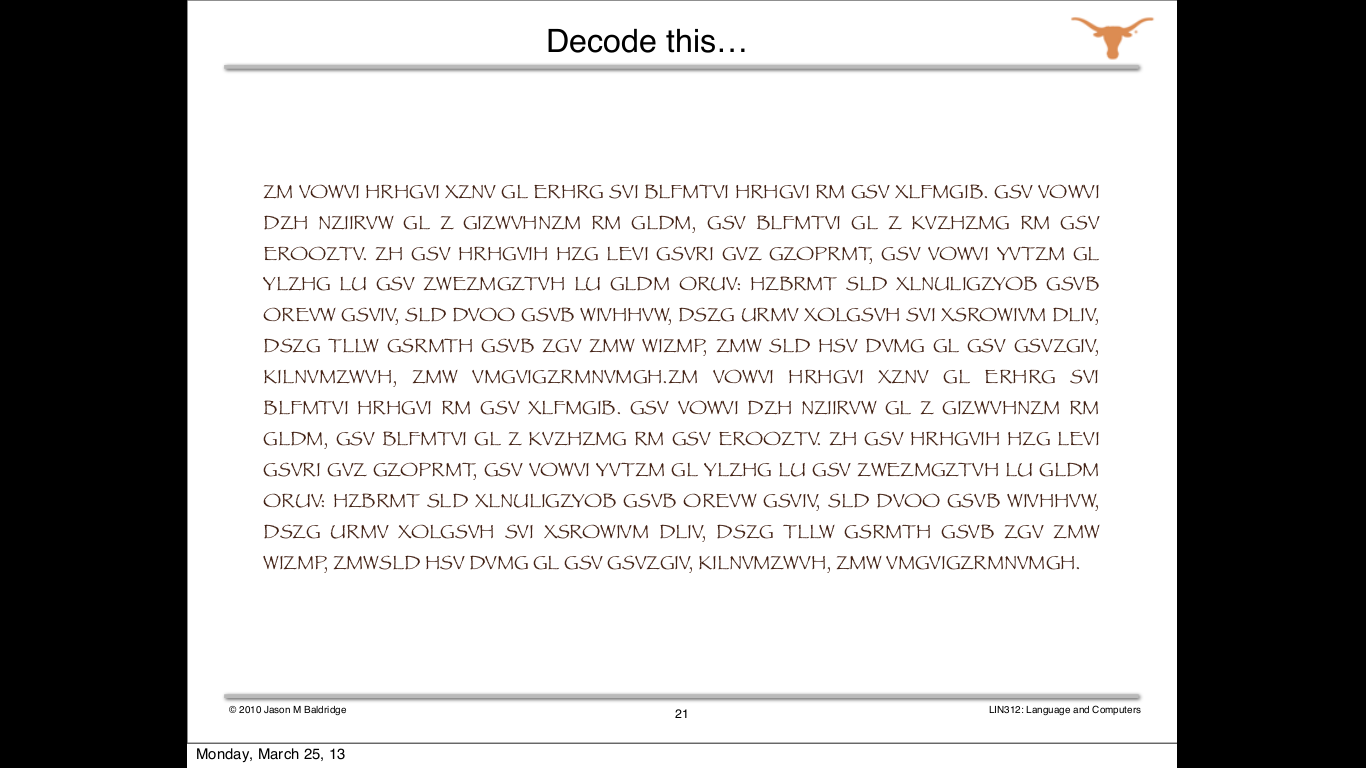
\includegraphics[width=0.9\textwidth]{brew.png}
\end{frame}

\begin{frame}
\frametitle{How to solve systematically?-1}
\begin{enumerate}
\item Make a table of characters
\item focus on a few common words, spot a few words. get a letter by letter mapping from there.
\item Chris Brew's slides (62--72)
\end{enumerate}
\end{frame}

\begin{frame}
\frametitle{How to solve systematically? -2}
\begin{enumerate}
\item Calculate frequencies of characters in the cipher
\item Compare that with general frequency of characters in English.
\item Roughly, the order of frequencies should be the same.
\end{enumerate} \pause
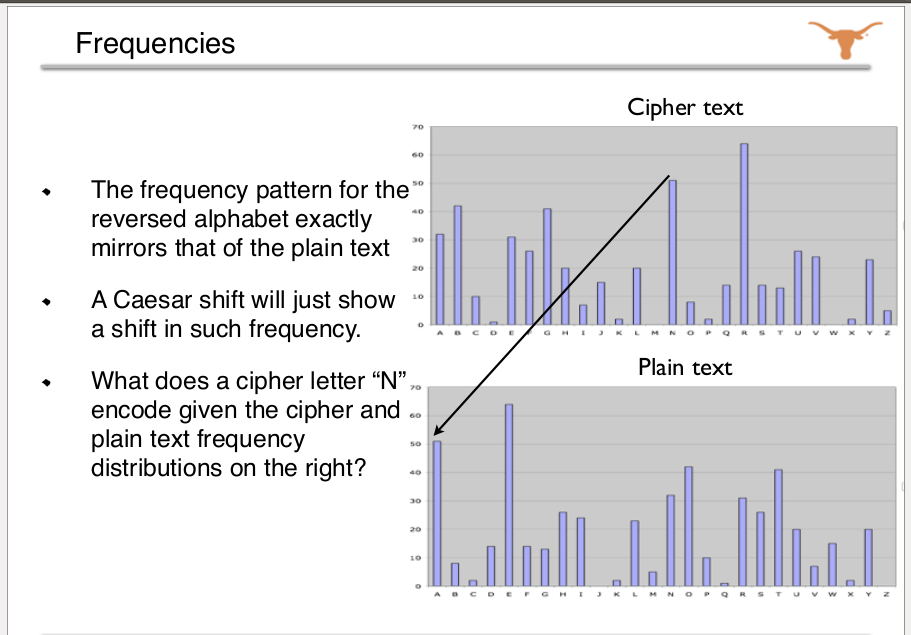
\includegraphics[width=0.9\textwidth]{frequencies.png}
\end{frame}

\begin{frame}
\frametitle{one-one mapping??}
\begin{enumerate}
\item Assumption in previous slides is that we have a one-one mapping between letters in a language.
\item One-one mapping (mono alphabetic) based cipher is easy to decipher with word spotting and frequencies.
\item So, there are poly-alphabetic ciphers (where there is one-to-many mapping, depending on context!)
\item example: \url{https://goo.gl/D9dXIU}
\end{enumerate}
\end{frame}
%Assumption: one character maps only to one other character - not always the case!!!

\begin{frame}	
\frametitle{Today's attendance exercise}
Try to figure out what this message is, following the ideas we discussed.
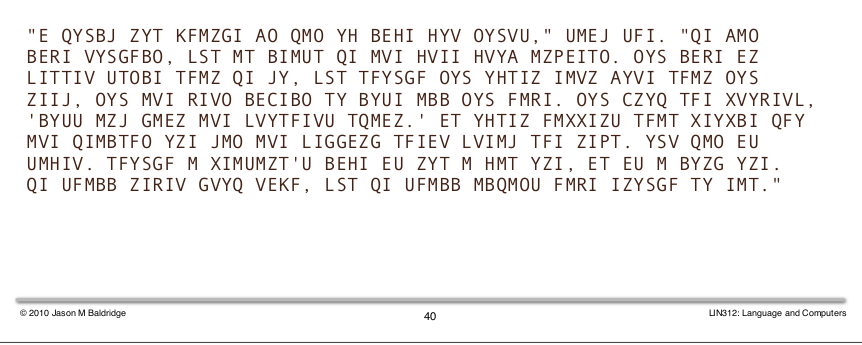
\includegraphics[width=0.9\textwidth]{16octexercise.png}
\pause Hint: U is perhaps S (only letter after an apostrophe)
\end{frame}

%Use brew's exercise.

\end{document}



